% Für Bindekorrektur als optionales Argument "BCORfaktormitmaßeinheit", dann
% sieht auch Option "twoside" vernünftig aus
% Näheres zu "scrartcl" bzw. "scrreprt" und "scrbook" siehe KOMA-Skript Doku
\documentclass[12pt,a4paper,titlepage,headinclude,bibtotoc]{scrartcl}


%---- Allgemeine Layout Einstellungen ------------------------------------------

% Für Kopf und Fußzeilen, siehe auch KOMA-Skript Doku
\usepackage[komastyle]{scrpage2}
\pagestyle{scrheadings}
\automark[section]{chapter}
\setheadsepline{0.5pt}[\color{black}]

%keine Einrückung
\parindent0pt

%Einstellungen für Figuren- und Tabellenbeschriftungen
\setkomafont{captionlabel}{\sffamily\bfseries}
\setcapindent{0em}


%---- Weitere Pakete -----------------------------------------------------------
% Die Pakete sind alle in der TeX Live Distribution enthalten. Wichtige Adressen
% www.ctan.org, www.dante.de

% Sprachunterstützung
\usepackage[ngerman]{babel}

% Benutzung von Umlauten direkt im Text
% entweder "latin1" oder "utf8"
\usepackage[utf8]{inputenc}

% Pakete mit Mathesymbolen und zur Beseitigung von Schwächen der Mathe-Umgebung
\usepackage{latexsym,exscale,amssymb,amsmath}

% Weitere Symbole
\usepackage[nointegrals]{wasysym}
\usepackage{eurosym}

% Anderes Literaturverzeichnisformat
%\usepackage[square,sort&compress]{natbib}

% Für Farbe
\usepackage{color}

% Zur Graphikausgabe
%Beipiel: \includegraphics[width=\textwidth]{grafik.png}
\usepackage{graphicx}

% Text umfließt Graphiken und Tabellen
% Beispiel:
% \begin{wrapfigure}[Zeilenanzahl]{"l" oder "r"}{breite}
%   \centering
%   \includegraphics[width=...]{grafik}
%   \caption{Beschriftung} 
%   \label{fig:grafik}
% \end{wrapfigure}
\usepackage{wrapfig}

% Mehrere Abbildungen nebeneinander
% Beispiel:
% \begin{figure}[htb]
%   \centering
%   \subfigure[Beschriftung 1\label{fig:label1}]
%   {\includegraphics[width=0.49\textwidth]{grafik1}}
%   \hfill
%   \subfigure[Beschriftung 2\label{fig:label2}]
%   {\includegraphics[width=0.49\textwidth]{grafik2}}
%   \caption{Beschriftung allgemein}
%   \label{fig:label-gesamt}
% \end{figure}
\usepackage{subfigure}

% Caption neben Abbildung
% Beispiel:
% \sidecaptionvpos{figure}{"c" oder "t" oder "b"}
% \begin{SCfigure}[rel. Breite (normalerweise = 1)][hbt]
%   \centering
%   \includegraphics[width=0.5\textwidth]{grafik.png}
%   \caption{Beschreibung}
%   \label{fig:}
% \end{SCfigure}
\usepackage{sidecap}

% Befehl für "Entspricht"-Zeichen
\newcommand{\corresponds}{\ensuremath{\mathrel{\widehat{=}}}}

%Für chemische Formeln (von www.dante.de)
%% Anpassung an LaTeX(2e) von Bernd Raichle
\makeatletter
\DeclareRobustCommand{\chemical}[1]{%
  {\(\m@th
   \edef\resetfontdimens{\noexpand\)%
       \fontdimen16\textfont2=\the\fontdimen16\textfont2
       \fontdimen17\textfont2=\the\fontdimen17\textfont2\relax}%
   \fontdimen16\textfont2=2.7pt \fontdimen17\textfont2=2.7pt
   \mathrm{#1}%
   \resetfontdimens}}
\makeatother

%Si Einheiten
\usepackage{siunitx}

%c++ Code einbinden
\usepackage{listings}
\lstset{numbers=left, numberstyle=\tiny, numbersep=5pt}

%errorFkt
\newcommand{\erf}{\ensuremath{\text{erf}}}

%Differential
\newcommand{\dif}{\ensuremath{\mathrm{d}}}

%Boxen,etc.
\usepackage{fancybox}
\usepackage{empheq}

%Fußnoten auf gleiche Seite
\interfootnotelinepenalty=1000


\begin{document}

\begin{titlepage}
\centering
\textsc{\Large Anfängerpraktikum der Fakultät für
  Physik,\\[1.5ex] Universität Göttingen}

\vspace*{4.2cm}

\rule{\textwidth}{1pt}\\[0.5cm]
{\huge \bfseries
  Spezifische Wärme der Luft und Gasthermometer\\[1.5ex]
  Protokoll:}\\[0.5cm]
\rule{\textwidth}{1pt}

\vspace*{2.0cm}

\begin{Large}
\begin{tabular}{ll}
Praktikant:
	&  Skrollan Detzler\\
 	&  Felix Kurtz\\
% 	&  Michael Lohmann\\
%	&  Kevin Lüdemann\\

  E-Mail: 
	&  skrollan.detzler@stud.uni-goettingen.de\\
	&  felix.kurtz@stud.uni-goettingen.de\\
%	& m.lohmann@stud.uni-goettingen.de\\
	
%	&  kevin.luedemann@stud.uni-goettingen.de\\

 Betreuer: & Martin Ochmann\\
 Versuchsdatum: & 02.06.2014\\
\end{tabular}
\end{Large}

\vspace*{0.8cm}

\begin{Large}
\fbox{
  \begin{minipage}[t][2.5cm][t]{6cm} 
    Testat:
  \end{minipage}
}
\end{Large}

\end{titlepage}

\tableofcontents

\newpage

\section{Einleitung}
\label{sec:einleitung}
Der erste Teil des Versuches dient der Bestimmung des absoluten Temperatur-Nullpunktes, eine der wichtigsten Naturkonstanten in der Thermodynamik.
Dies geschieht mithilfe eines Gasthermometers.\\
Im zweiten Teil bestimmt man die spezifische Wärme von Luft.

\section{Theorie}
\label{sec:theorie}
\subsection{Gasthermometer}
\begin{align}
	p=p_L+\Delta p
\end{align}
Gay-Lussac und Boyle-Mariotte
\begin{align}
	p(\vartheta)=p_0 [1+\beta\vartheta]\\
	V(\vartheta)=V_0 [1+\beta\vartheta]
\end{align}
\begin{align}
	p\cdot V=\text{const}.
\end{align}
\begin{align}
	\beta=1/(273.15 \si{\celsius})
\end{align}

\subsection{Spezifische Wärme der Luft}
allgemeine Gasgleichung
\begin{align}
	p \cdot V = nRT = Nk_B T 
\end{align}
1.Hauptsatz der Wärmelehre
\begin{align}
	\dif Q = \dif U+\dif W
\end{align}
innere Energie
\begin{align}
	U=\frac{f}{2} k_B T
\end{align}
Energie eines Kondensators
\begin{align}
	W=\frac{1}{2}CU^2
\end{align}

\section{Durchführung}
\label{sec:durchfuehrung}
\subsection{Gasthermometer}
\begin{figure}[!htb]
 \centering
 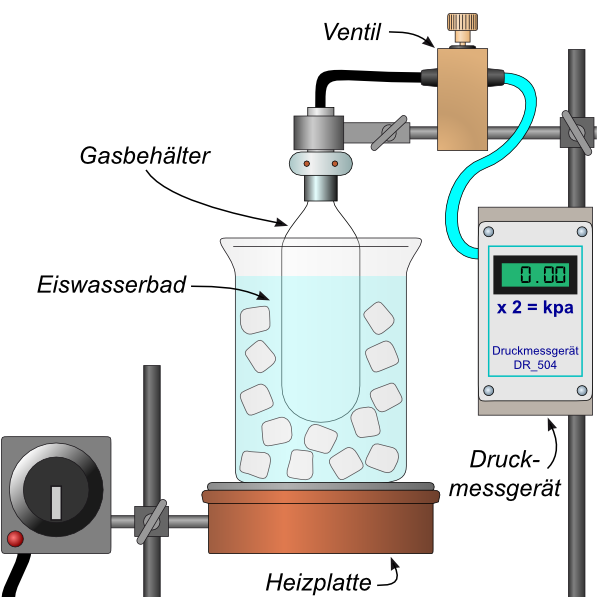
\includegraphics{GasthermometerSkizze.jpg}
 \caption{Skizze des Gasthermometers \cite{lp}}
 \label{fig:GTSkizze}
\end{figure}

Zuerst wird das Ventil des Druckmessgerätes geöffnet, um im Gaskolben Umgebungsdruck herzustellen.
Nun wird der Glaskolben durch Eiswasser auf etwa $0^\circ$ C herunter gekühlt.
Das Druckmessgerät sollte ungefähr 0 kPa anzeigen, da es nur Differenzen zum Umgebungsdruck angibt. Danach das Ventil schließen.\\
Nun wird die Heizplatte angeschaltet und damit das den Glaskolben umgebende Wasser auf bis zu $100^\circ$ C erhitzt.
Dabei misst man in $5^\circ$ C Schritten den Überdruck im Kolben.
Es ist also immer auf das Thermometer zu achten.
Außerdem muss das Wasser ständig umgerührt werden, um eine möglichst homogene Temperatur sicherzustellen.
Ferner sollte man bei hohen Temperaturen aufpassen, dass man sich nicht verbrüht.
Dann wird die Platte abgeschaltet, das Gefäß von dieser herunterbewegt und das Wasser mit Eis heruntergekühlt.
Dabei muss auf die Menge geachtet werden, da man auch beim Abkühlen den Druck in Abhängigkeit von der Temperatur messen soll.
Deshalb ist auch das Umrühren unerlässlich.
Des weiteren muss dafür gesorgt werden, dass das überlaufende Wasser aufgefangen wird. 
\subsection{Spezifische Wärme der Luft}
\begin{figure}[!htb]
 \centering
 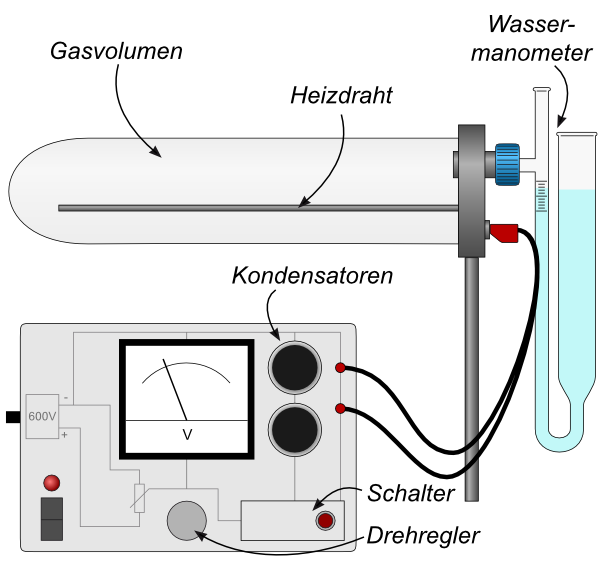
\includegraphics{SpezWaermeSkizze.jpg}
 \caption{schematischer Aufbau, um die spezifische Wärme von Luft zu messen \cite{lp}}
 \label{fig:SWLSkizze}
\end{figure}
Zuerst wird der Kondensator mit einer voreingestellten Spannung zwischen 100V und 500V geladen.
Diesen entlädt man daraufhin über den Heizdraht, während man parallel den Maximalausschlag des Manometers abliest.
Dieser Vorgang wird für mehrere Spannungen je dreimal wiederholt.
Zwischen den Messungen wird der Zylinder belüftet.

\section{Auswertung}
\label{sec:auswertung}


\section{Diskussion}
\label{sec:diskussion}

\section{Anhang}

\begin{thebibliography}{100}

\bibitem{gerthsen}
	\textsc{Dieter Meschede} (2010): \emph{Gerthsen Physik}, 24. Auflage, Springer Heidelberg
Dordrecht London New York

\bibitem{demtroeder}
\textsc{Wolfgang Demtröder} (2008): \emph{Experimentalphysik 1 - Mechanik und Wärme}, 5. Auflage, Springer Berlin, Heidelberg

\bibitem{lp} 
	\emph{Lehrportal der Universität Göttingen, Spezifische Wärme der Luft und Gasthermometer},
  http://lp.uni-goettingen.de/get/text/3643, abgerufen 23.07.14 11:13 Uhr

\end{thebibliography}


\end{document}
